\documentclass[12pt, a4paper]{article}

\usepackage[utf8]{inputenc}
\usepackage[slovene]{babel}
\usepackage{graphicx}
\usepackage{amsmath}
\usepackage{amsfonts}
\usepackage{latexsym}
\usepackage{amssymb}
\usepackage{listings}



\begin{document}


\begin{titlepage}
    \center
    \textsc{\LARGE Univerza v Ljubljani}\\[0.6cm]
    \textsc{\Large Fakulteta za matematiko in fiziko}\\[0.6cm]
    
    {\huge\bfseries Vpliv dodatnih informacij na oceno pričakovanega trajanja in variance pri modelu PERT}\\[0.4cm]
    
    
    \vfill\vfill\vfill
    
    { Mykola Shafranov, Tine Markočič}
    
    { Januar, 2022}
    
    \vfill
    
\end{titlepage}
    
\tableofcontents
    
\newpage



\section{Opis problema}
Pri metodi PERT se za napoved trajanja projekta uporablja ocene trajanj posameznih opravil. 
Za ta se najpogosteje predpostavi, da imajo Beta porazdelitev na nekem intervalu $[a,b]$. 
Pri ocenah nas najbolj zanima pričakovano trajanje in varianca posameznega opravila. V klasičnem
modelu za ti oceni vzamemo
$$\mu_1 = \frac{a + 4M + b}{6}$$
$$\sigma_1^2 = \frac{(a + b)^2}{36}$$
kjer je $M$ najbolj verjetno trajanje. \\

V projektu bova preučila alternativne možnosti za ocene pričakovanega trajanja in variance opravil.
Pri tem si bova pomagala z izračuni in izpeljavami iz članka \cite{clanek}.


\section{Načrt dela}
\begin{itemize}
\item Generirati nameravava nekaj usmerjenih acikličnih grafov (ali pa bova poiskala kakšne realne primere), 
kjer vsako vozlišče predstavlja neko opravilo. Za vsako opravilo bova določila neko porazdelitev 
(verjetno beta) za njegovo trajanje. Po modelu PERT in njegovi modifikaciji - s pristopom s porazdelitvijo 
maksimalne entropije, ki je opisan v članku \cite{clanek}, bova določila pričakovano trajanje in varianco
vsakega opravila ter na podlagi tega določila kritično pot in pa njeno pričakovano trajanje in varianco.
\item Naredila bova večje število vzorcev, pri čemer bova vsakič za posamezno opravilo naključno določila 
njegovo trajanje glede na ustrezno porazdelitev, ter poračunala kritično pot in njeno trajanje po modelu CPM.
Nato bova preverila, kako se dobljeni rezultati skladajo z vrednostmi, dobljenimi z metodo PERT in pa z
njeno modifikacijo. To bova preverila s pomočjo ustreznih statističnih testov.
\end{itemize}

\newpage{}

\section{Potek dela}

Za začetek sva generirala nekaj usmerjenih acikličnih grafov, in nekatere iz njih tudi izbrala za najino nalogo. Izbrane grafe sva nato zapisala kot množico urejenih parov vozlišč $u$ in $v$. Nato sva vse izbrane grafe izrisala za boljšo predstavo. To kot tudi glavni program sva sprogramirala v programskem jeziku R.

Pri vsakem grafu določajo posamezna vozlišča vsako svoje opravilo, ki ima definirano najkrajše možno trajanje, najverjetnejše trajanje in pa najdaljše možno trajanje. V glavnem programu sva na začetku za vsako od opravil določila intervale za najkrajše in najdaljše možno trajanje, natančneje, za najkrajše možne čase sva izbrala interval $[2,8]$, za najdaljše pa $[15,25]$. Za najverjetnejše trajanje sva uporabila porazdelitev $B(p,q)$. Za parametra $p$ in $q$ sva določila meje v intervalu $(1,10)$, in ta parametra nato za vsako od opravil generirala. Nato sva lahko poračunala najverjetnejše trajanje za vsako od opravil.

\section{Funkcije}
S pomočjo naslednjih funkcij sva za vsak graf določila kritično pot po poljubni metodi. Na posameznem 
grafu sva za vsako vozlišče s funkcijama \texttt{seznam\_predhodnikov} in \texttt{seznam\_sosedov} 
določila njegove predhodnike in sosede. \\
Nato sva s funkcijo \texttt{prehod\_naprej} določila najzgodnejše začetke posameznih opravil. Funkcija teče od prvega do zadnjega opravila.
\begin{lstlisting}[language=R]
prehod_naprej = function(predhodniki, cas){
  n_tock = length(predhodniki)
  t = rep(0,n_tock)
  predniki_na_poti = c(0, rep(1,n_tock-1))
  for (i in 2:n_tock) {
    for (j in predhodniki[[i]])
      if(t[j] + cas[j] > t[i]){
        t[i] = t[j] + cas[j]
        predniki_na_poti[i] = j
      }
  }
  list(t, predniki_na_poti)
}
\end{lstlisting}

Podobno nam funkcija \texttt{prehod\_nazaj} določi najkasnejše začetke opravil, tako da začne pri zadnjem in teče do prvega vozlišča grafa.
\begin{lstlisting}[language=R]
prehod_nazaj = function(sosedi,t, cas){
  n_tock = length(sosedi)
  T = rep(t[n_tock],n_tock)
  for (i in (n_tock-1):1) {
    for (j in sosedi[[i]])
      if(T[j] - cas[i] < T[i])
        T[i] = T[j] - cas[i]
  }
  T
}   
\end{lstlisting}

Funkcija \texttt{k\_pot} nam preko seznama prednikov vozlišč določi kritično pot grafa.
\begin{lstlisting}[language=R]
k_pot = function(predniki){
  n_tock = length(predniki)
  i = n_tock
  pot = c()
  while (i != 0){
    pot = c(i,pot)
    i = predniki[[i]]
  }
  pot
}
\end{lstlisting}

Na koncu sva pognala funkcijo \texttt{kriticna\_pot}, ki preko zgoraj navedenih funkcij poračuna kritično pot posameznega grafa ter izpiše najzgodnejše začetke $t$, najkasnejše začetke $T$, kritično pot in variance opravil.

\section{Modifikacije}
Zanima naju kakšne vrednosti lahko dobimo z različnimi ocenami pričakovanega trajanja in variance.
Vse modifikacije, ki sva se jih odločila analizirati, sva vzela iz članka \cite{clanek}. Te sva smiselno razdelila v dve kategoriji.

\subsection{Beta porazdelitev z dodatki}
\textbf{Klasičen PERT}\\
Najprej seveda klasična metoda, kjer sva vzela vrednosti $\mu_1$ in $\sigma_1$ iz Uvoda. Ti vrednosti
sta nama v analizi služila kot solidna in zanesljiva primerjava za ostale modifikacije.

\vspace{0,5cm}
\textbf{1. Modifikacija}\\
Izpeljana je iz odvoda in pričakovane vrednosti Beta porazdelitve po parametru $q$ in njene limite, ko gre $q$ proti $1$. Modifikacija je še posebej uporabna, ko za parametra porazdelitve velja zveza:$p = 1 + 2\frac{M - a}{b - a}$ in $q = 1 + 2\frac{b - M}{b - a}$. Naši oceni pa sta v tem primeru:
$$\mu_2 = \frac{a + 2M + b}{4}$$
$$\sigma_2^2 = \frac{(b + 2M - 3a)(3b - 2M - a)}{80}$$

\vspace{0,5cm}
\textbf{2. Modifikacija}\\
Do te modifikacije pridemo ob predpostavki, da je znana pričakovana vrednost porazdelitve in je enaka $\mu_1$. To nas privede do unikatne porazdelitve s parametra $p = 1 + 4\frac{M - a}{b - a}$ in $q = 1 + 4\frac{b - M}{b - a}$ in ocen:
$$\mu_3 = \mu_1$$
$$\sigma_3^2 = \frac{(b + 4M - 5a)(5b - 4M - a)}{252}$$

\vspace{0,5cm}
\textbf{3. Modifikacija}\\
Podobno kot v 2. Modifikaciji tu predpostavimo, da je znana varianca porazdelitve in je enaka $V$. Tu je najpogosteje analiziran primer, ko velja $V = \frac{(a + b)^2}{36}$. Pri tej modifikaciji pa je težje določiti oceno za pričakovano trajanje, saj je ta odvisna od parametra $q_{(V)}$, ki ga izračunamo iz kubične enačbe dane z znano varianco. Ta modifikacija je zato manj optimalna in pogosto izpuščena. Oceni sta:
$$\mu_4 = \frac{q_{(V)}M(b - a) + b(b + a -2M)}{q_{(V)}(b - a) + b + a - 2M}$$
$$\sigma_4^2 = \sigma_1^2$$


\subsection{Splošnejši primeri}
\textbf{4. Modifikacija}\\
Pri naslednjih dveh modifikacijah pozabimo na beta porazdelitev, saj so izpeljane na način, da ustrezajo za vsako porazdelitev, kjer lahko določimo M. Zanimivo je v tem primeru predlagana enaka ocena za pričakovano trajanje kot pri 1. Modifikaciji. Ocena za varianco pa je unikatna:
$$\mu_5 = \mu_2$$
$$\sigma_5^2 = \frac{(a - b)^2 + 6(a - M)^2 + 6(b - M)^2}{144}$$

\vspace{0,5cm}
\textbf{5. Modifikacija}\\
Pri naši zadnji modifikaciji pride še do dodatne posplošitve, in sicer tu ni več potrebno poznati vrednosti M. Gre za to, da poznamo nek podinterval $[a_1, b_1]$ intervala $[a, b]$ in vemo, da je verjetnost, da bo vrednost trajanja opravila na njem, enaka $\epsilon$. To nam da nekoliko kompleksnejši oceni:
$$\mu_6 = \frac{\epsilon}{2}(a_1 + b_1) + \frac{1 - \epsilon}{2}\frac{b^2 - a^2 - b_1^2 + a_1^2}{b - a - b_1 + a_1}$$
$$\sigma_6^2 = \frac{(1 - \epsilon)(b^3 - a^3 - b_1^3 + a_1^3)}{3(b - a - b_1 + a_1)} + \epsilon(b_1^2 + a_1^2 + a_1b_1) - \mu_6^2$$

\vspace{0,5cm}
\textbf{Model CPM}\\
Pri vseh različnih metodah PERT, ki jim imamo na razpolago, pa se nama je zdelo zanimivo te primerjati še z modelom CPM. Ta seveda nima ne računa vrednosti varianc, zato sva določila le oceno za pričakovano trajanje, in sicer:
$$cas = M$$


\newpage{}

\section{Rezultati}

Za vsako od metod sva za rezultate vzela vzorec velikosti 100. Primerjala sva vrednosti najverjetnejših trajanj projektov po kritičnih poteh in pa povprečne variance projektov. V poročilu sva se osredotočila na rezultate pri 2. grafu.

\begin{center}
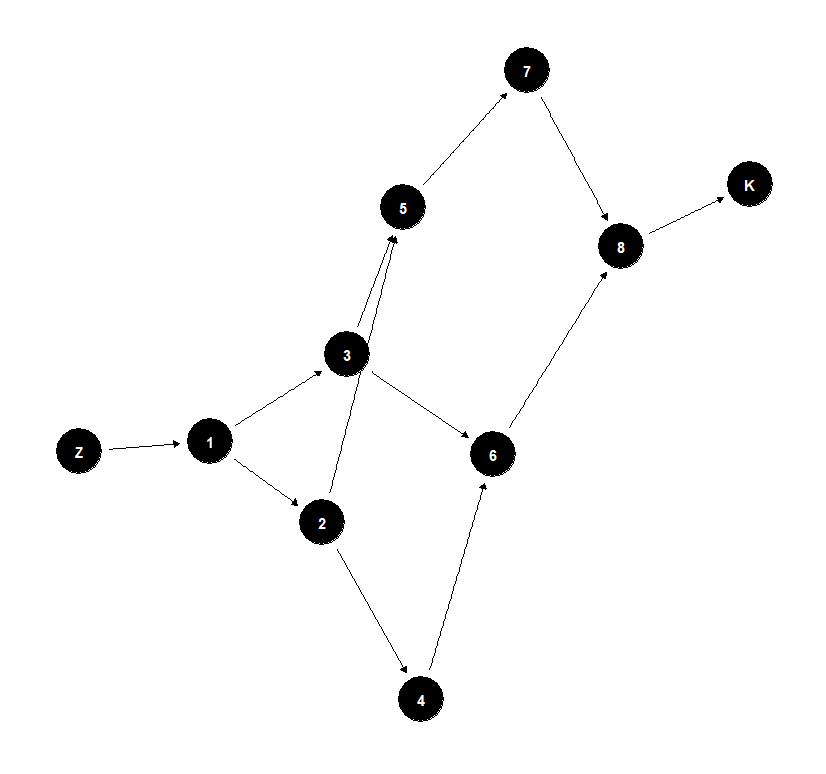
\includegraphics[scale=0.55]{2_graf.png}
\end{center}

Opazila sva, da so povprečna trajanja projekta pri vseh modifikacijah skorajda enaka. 
\begin{center}
\begin{tabular}{| l | l |}
\hline
Metoda & Povprečno trajanje projekta \\
\hline
PERT & 57.965927 \\
\hline
$1$. modifikacija & 57.974445 \\
\hline
$2$. modifikacija & 57.965927 \\
\hline
$4$. modifikacija & 57.974445 \\
\hline
CPM & 57.948891 \\
\hline
\end{tabular}
\end{center}
Glede na to, da so najverjetnejša trajanja projekta pri vseh metodah skoraj enaka, lahko sklepamo, da so vse metode uporabne in dokaj učinkovite.

Variance pa so se na drugi strani med seboj kar dosti razlikovale.
\begin{center}
\begin{tabular}{| l | l |}
\hline
Metoda & Povprečna varianca projekta \\
\hline
PERT & 25.888888 \\
\hline
$1$. modifikacija & 88.686644 \\
\hline
$2$. modifikacija & 29.940122 \\
\hline
$4$. modifikacija & 30.279978 \\
\hline
\end{tabular}
\end{center}
Večja varianca pomeni, da so rezultati bolj razpršeni, in to se najbolj pozna pri 1. modifikaciji. Pričakovano je najnižja varianca pri osnovni metodi PERT. Pri CPM-ju pa, kot sva že omenila, variance sploh ne določamo.

\section{Zaključek}
Izkazalo se je, da lahko z vsemi metodami dobro napovedujemo trajanje projekta, kljub temu da so zasnovane na različnih predpostavkah. Za naprej bi bilo zanimivo preveriti kako metode delujejo na drugih porazdelitvah. Prav tako, bi lahko preverili še 3. in 5. Modifikacijo, ki nam jih zaradi njune zahtevnejše izpeljave ni uspelo vključiti v analizo.


\newpage{}

\begin{thebibliography}{9}
\bibitem{clanek}
A.~Hernández-Bastida in M.P.~Fernández-Sánchez, \emph{How adding new information modifies the estimation of
the mean and the variance in PERT: a maximum entropy distribution approach}, Ann. Oper. Res. 274(1-2): (2019) 291--308.

\bibitem{spletni-vir}
A.~Žitnik, \emph{Spletna učilnica OR}, v: Zapiski s predavanj, verzija 27.~5.~2021, [ogled 3.~1.~2022], dostopno na {https://ucilnica2021.fmf.uni-lj.si}.

\end{thebibliography}


\end{document}